\chapter{Next Steps for my PhD}

My work so far has been on two very different projects centering around RNA regulation in models of ALS/FTD. The cryptic splicing project in TDP-43 was based on public data, which allowed for rapid progress and the ability to replicate my conclusions across multiple experiments. However, brute force knockdown of TDP-43 is a very crude model of disease and the project suffered from the low quality of RNA-seq data and the inability to validate the mechanism with a wet lab collaborator. The FUS $\Delta$14 mouse project however offers up a humanised mouse model where disease-like changes occur progressively. There is much appetite from Anny Devoy and from the lab of Pietro Fratta to continue investigations into the mechanism of the mutation's effect on RNA regulation.\\ 

Over the remainder of my PhD I plan to upgrade the RNA-seq pipeline to use state-of-the-art splicing analysis software. I will then apply this pipeline to better understand the changes in splicing that occur in the FUS $\Delta$14 mouse, as well as in new data being generated on the mutation's impact on mRNA transport and translation. I will also apply the splicing pipeline to two opposing \textit{TARDBP} mutant mice and compare the results with existing TDP-43 knockdown data. To continue the cryptic splicing project I will screen the large ENCODE cohort of RNA-binding proteins for cryptic exon repression and then look for evidence of cryptic splicing in ALS/FTD patient brains. 
	

\section{Developing a full-featured splicing analysis pipeline}
Since I started work on \textit{CryptEx} in October 2015 there have several major advancements in algorithms to analyse differential splicing from RNA-seq data. This has been enabled by improvement in the quality of RNA-seq data. \textit{CryptEx} and the underlying \textit{DEXSeq} approach were designed to work on all qualities of data going back to low depth, short read datasets generated in 2010. So while it has been useful for the TDP-43 project I believe I should make use of the state-of-the-art tools now available. Dr Kitty Lo and I have installed and assessed the latest advances in RNA-seq analysis algorithms. We can group software packages into one of four categories based on what they consider to be the fundamental unit of differential splicing. All of these modern algorithms require paired end data with high coverage and long reads to maximise the information available.

\subsection{Transcript quantifiers}
These compare abundances at the transcript level and rely on a curated list of known transcripts. Sequencing reads are then probabilistally assigned to a each transcript. This can be done extremely quickly in the case of pseudoaligners like \textit{Kallisto} \citep{Bray2015}. Transcript assembly algorithms like \textit{Stringtie} \citep{Pertea2015} can even assemble reads into novel transcripts. These algorithms require long reads for enough splicing information and very dependent on the list of transcripts they are given. Some genes can generate hundreds of very similar transcript isoforms or overlap with other genes and so these methods will struggle to accurately assign reads to them.

\subsection{Exon quantifiers}
These algorithms are typified by the \textit{DEXSeq} approach \citep{Anders2012}, where the transcripts are flattened to create a set of unique exon "bins".  As the bins themselves may not actually be an exon it makes the results difficult to interpret, although this has been lessened in a new software package called \textit{JunctionSeq} \citep{Hartley2015}, which also quantifies splice junctions and can pick up novel splice junctions. As they consider the whole gene they are sensitive to poorly annotated genes and extreme biases in coverage.

\subsection{Local splicing event quantifiers}
These algorithms work by comparing differences in splice junctions across the body of a gene while being agnostic to transcript annotations, allowing for the detection of novel events. These algorithms then establish different categories of possible events such as cassette exons, exon extensions, intron retention and alternate first or last exons. Each event is then tested for differences in inclusion/exclusion across conditions. This approach has been implemented in the \textit{SUPPA} \citep{Alamancos2015}, \textit{SGSeq} \citep{Goldstein2016} and \textit{MAJIQ} \citep{Vaquero-Garcia2016} packages. These packages, while providing a clear output of different splicing events, struggle to determine splicing events such as tandem 3'UTR changes which can only be differentiated by read coverage and not splice junctions. 

\subsection{Annotation-free quantifiers}
The fourth and final class of algorithm don't depend on any transcript annotation at all. The \textit{derFinder} package \citep{ColladoTorres2015} assesses changes in read coverage between samples, which is particularly useful in looking for novel non-coding RNA species or in the aforementioned tandem 3'UTR problem. The \textit{LeafCutter} package \citep{Li2016} looks for differentially used splice junctions independently of annotation and has shown that across a set of tissues around 30\% of the high confidence splice junctions recovered are novel to any annotation database.\\

Dr Lo and I will create a pipeline that implements a combination of the above approaches to gain a full picture of splicing dysregulation in the FUS $\Delta$14 mouse and also in a different set of TDP-43 mutant mice.


%%
%%Stringtie is the successor to Cufflinks for assembling transcripts \citep{Pertea2015}.
%%
%%The DEXSeq methodology suffers from discarding the valuable information given by splice junctions and that has now been incorporated into the JunctionSeq package . 
%%Categorising splicing changes
%%SGSeq - what good for? \citep{Goldstein2016}
%%SUPPA \citep{Alamancos2015}
%%Annotation-free quantification of splicing derFinder \citep{ColladoTorres2015}
%%LeafCutter \citep{Li2016}
%%
%%In collaboration with Dr Kitty Lo, we will build a state-of-the-art splicing pipeline.

\section{RNA dysregulation in two opposing \textit{TARDBP} mutant mice}

The lab of Dr Pietro Fratta have generated two mouse lines with mutations in TDP-43 from a large mutagenesis screen \citep{Ricketts2014}. One line, F210I, contains a mutation in the second RNA recognition motif and another, M323K contains a mutation in the C-terminal low complexity domain which is where the majority of ALS patient mutations occur \citep{Sreedharan2008-xv}. The F210I mutation is embryonic lethal in homozygosity whereas the M323K mutation appears to lead to a progressive motor neuron loss in adult mice. The Fratta lab has generated high quality RNA-seq data for the embryonic F210I and the adult M323K mice. Kitty Lo and I will apply our state-of-the-art splicing pipeline to investigate the splicing changes and compare them to existing TDP-43 knockdown data used in the cryptic splicing project. 
Preliminary analysis has demonstrated a large number of cryptic exons in the F210I embryonic mice that overlap with the TDP-43 knockdown data from \citep{Polymenidou2011}. The lab has also generated iCLIP data by precipitating the RNA targets of the two mutant proteins (Dr Agnieszka Ule and Prasanth Sivakumar). It will be very interested to see how the two mutations alter TDP-43's splicing functionality and how that relates to toxicity and neurodegeneration.

\section{Dissecting the role of FUS in mRNA transport and translation}
The gene expression analysis of the FUS $\Delta$14 mice showed a general downregulation of ribosomal mRNAs. This is interesting as FUS has been noted to play a role in mRNA transport outside of the nucleus for local translation \citep{Kanai2004,Fujii2005} as well as modulating translation by transporting RNA to translationally active granules \citep{Yasuda2013} or to translationally silent stress granules \citep{Bosco2010}. In the light of this, the lab of Pietro Fratta want to observe the effect of the $\Delta$14 FUS mutation on both RNA transport in axons and the modulation of translation. 
The impact of the FUS $\Delta$14 mutation on axonal transport will be observed by performing RNA-seq on spatially separated samples of motor neuron cell bodies and axons. This approach has been successful in wildtype neuronal cells \citep{Taliaferro2016}, where specific splicing isoforms were enriched in axons compared to cell bodies. This work will be carried out by Dr Nicol Birsa. I will process and analyse RNA-seq libraries created from both the axons and the cell bodies of wildtype and FUS $\Delta14$ motor neurons. I will try to compare axon-enriched mRNAs between wildtype and disease to uncover which mRNAs are affected by the FUS mutation, either by changes in localisation or changes in the splicing isoform for that gene.

Polysome profiling involves immuno-tagging of a specific ribosomal protein in a specific cell type. These tagged ribosomes can be pulled down and the bound RNA can be sequenced to determine the RNA species and isoform \citep{Shigeoka2016}. This can then be compared to a background sequencing library to demonstrate an enrichment of a set of RNAs bound to ribosomes in mouse motor neurons carrying either the wildtype or mutant FUS. This work will be carried out by Dr Agnieszka Ule. I will then analyse RNA-seq libraries created from the ribosome-bound RNA to look for changes in translation between the wildtype and FUS $\Delta14$ motor neurons.

By combining the two datasets I should be able to build a model of how the FUS $\Delta$14 mutations affects both the transport and translation of mRNAs. 

\section{Screening the \textit{ENCODE} RNA-seq cohort for cryptic splicing}
In chapter 3 I made use of publicly available RNA-seq data generated by the \textit{ENCODE} consortium (\url{www.encodeproject.com}) which has performed shRNA knockdown experiments on over 150 RNA-binding proteins, including the ALS/FTD-linked proteins TDP-43 and FUS, as well as MATR3, hnRNPA1, hnRNPA2B1 and TAF15. My cryptic splicing project concluded that TDP-43 but not FUS plays a role in repressing nonconserved elements of the genome from being included into transcripts but whether or not this occurs in other ALS-linked genes is unknown. There has not been a large screen of cryptic splicing across multiple proteins as previous studies have focussed on individual candidates: hnRNP C \citep{Zarnack2013-nv}, PTBP1/2 \citep{Ling2016} and RBM17 \citep{Tan07102016}.
I therefore plan to download and align all shRNA knockdown data from ENCODE and run the data through both my own cryptic splicing pipeline (\textit{Cryptex}) and through a number of different algorithms that quantify novel splicing. I have already processed the data from the previously mentioned proteins and compared the number of high confidence cryptic exons discovered by \textit{Cryptex} with the strength of the knockdown of the target gene calculated by \textit{DESeq2} \citep{Love2014} (Figure 5.1). The results are promising as it appears that MATR3, TAF15 and hnRNPA2B1 knockdown leads to inclusion of a large number of cryptic exons, but only in experiments with a sufficiently strong knockdown. The results illustrate the variability in shRNA knockdown throughout the cohort. In TDP-43 around 70 cryptic exons can be seen in the K562 leukaemia cell line but fewer than 10 can be observed in the HepG2 liver carcinoma cell line, which has a much poorer knockdown. Screening the ENCODE cohort for cryptic splicing may uncover a new set of cryptic exon repressing RNA-binding proteins, or may even show that cryptic splicing repression is a common function of many RNA-binding proteins. 

\begin{figure}
	\begin{center}
		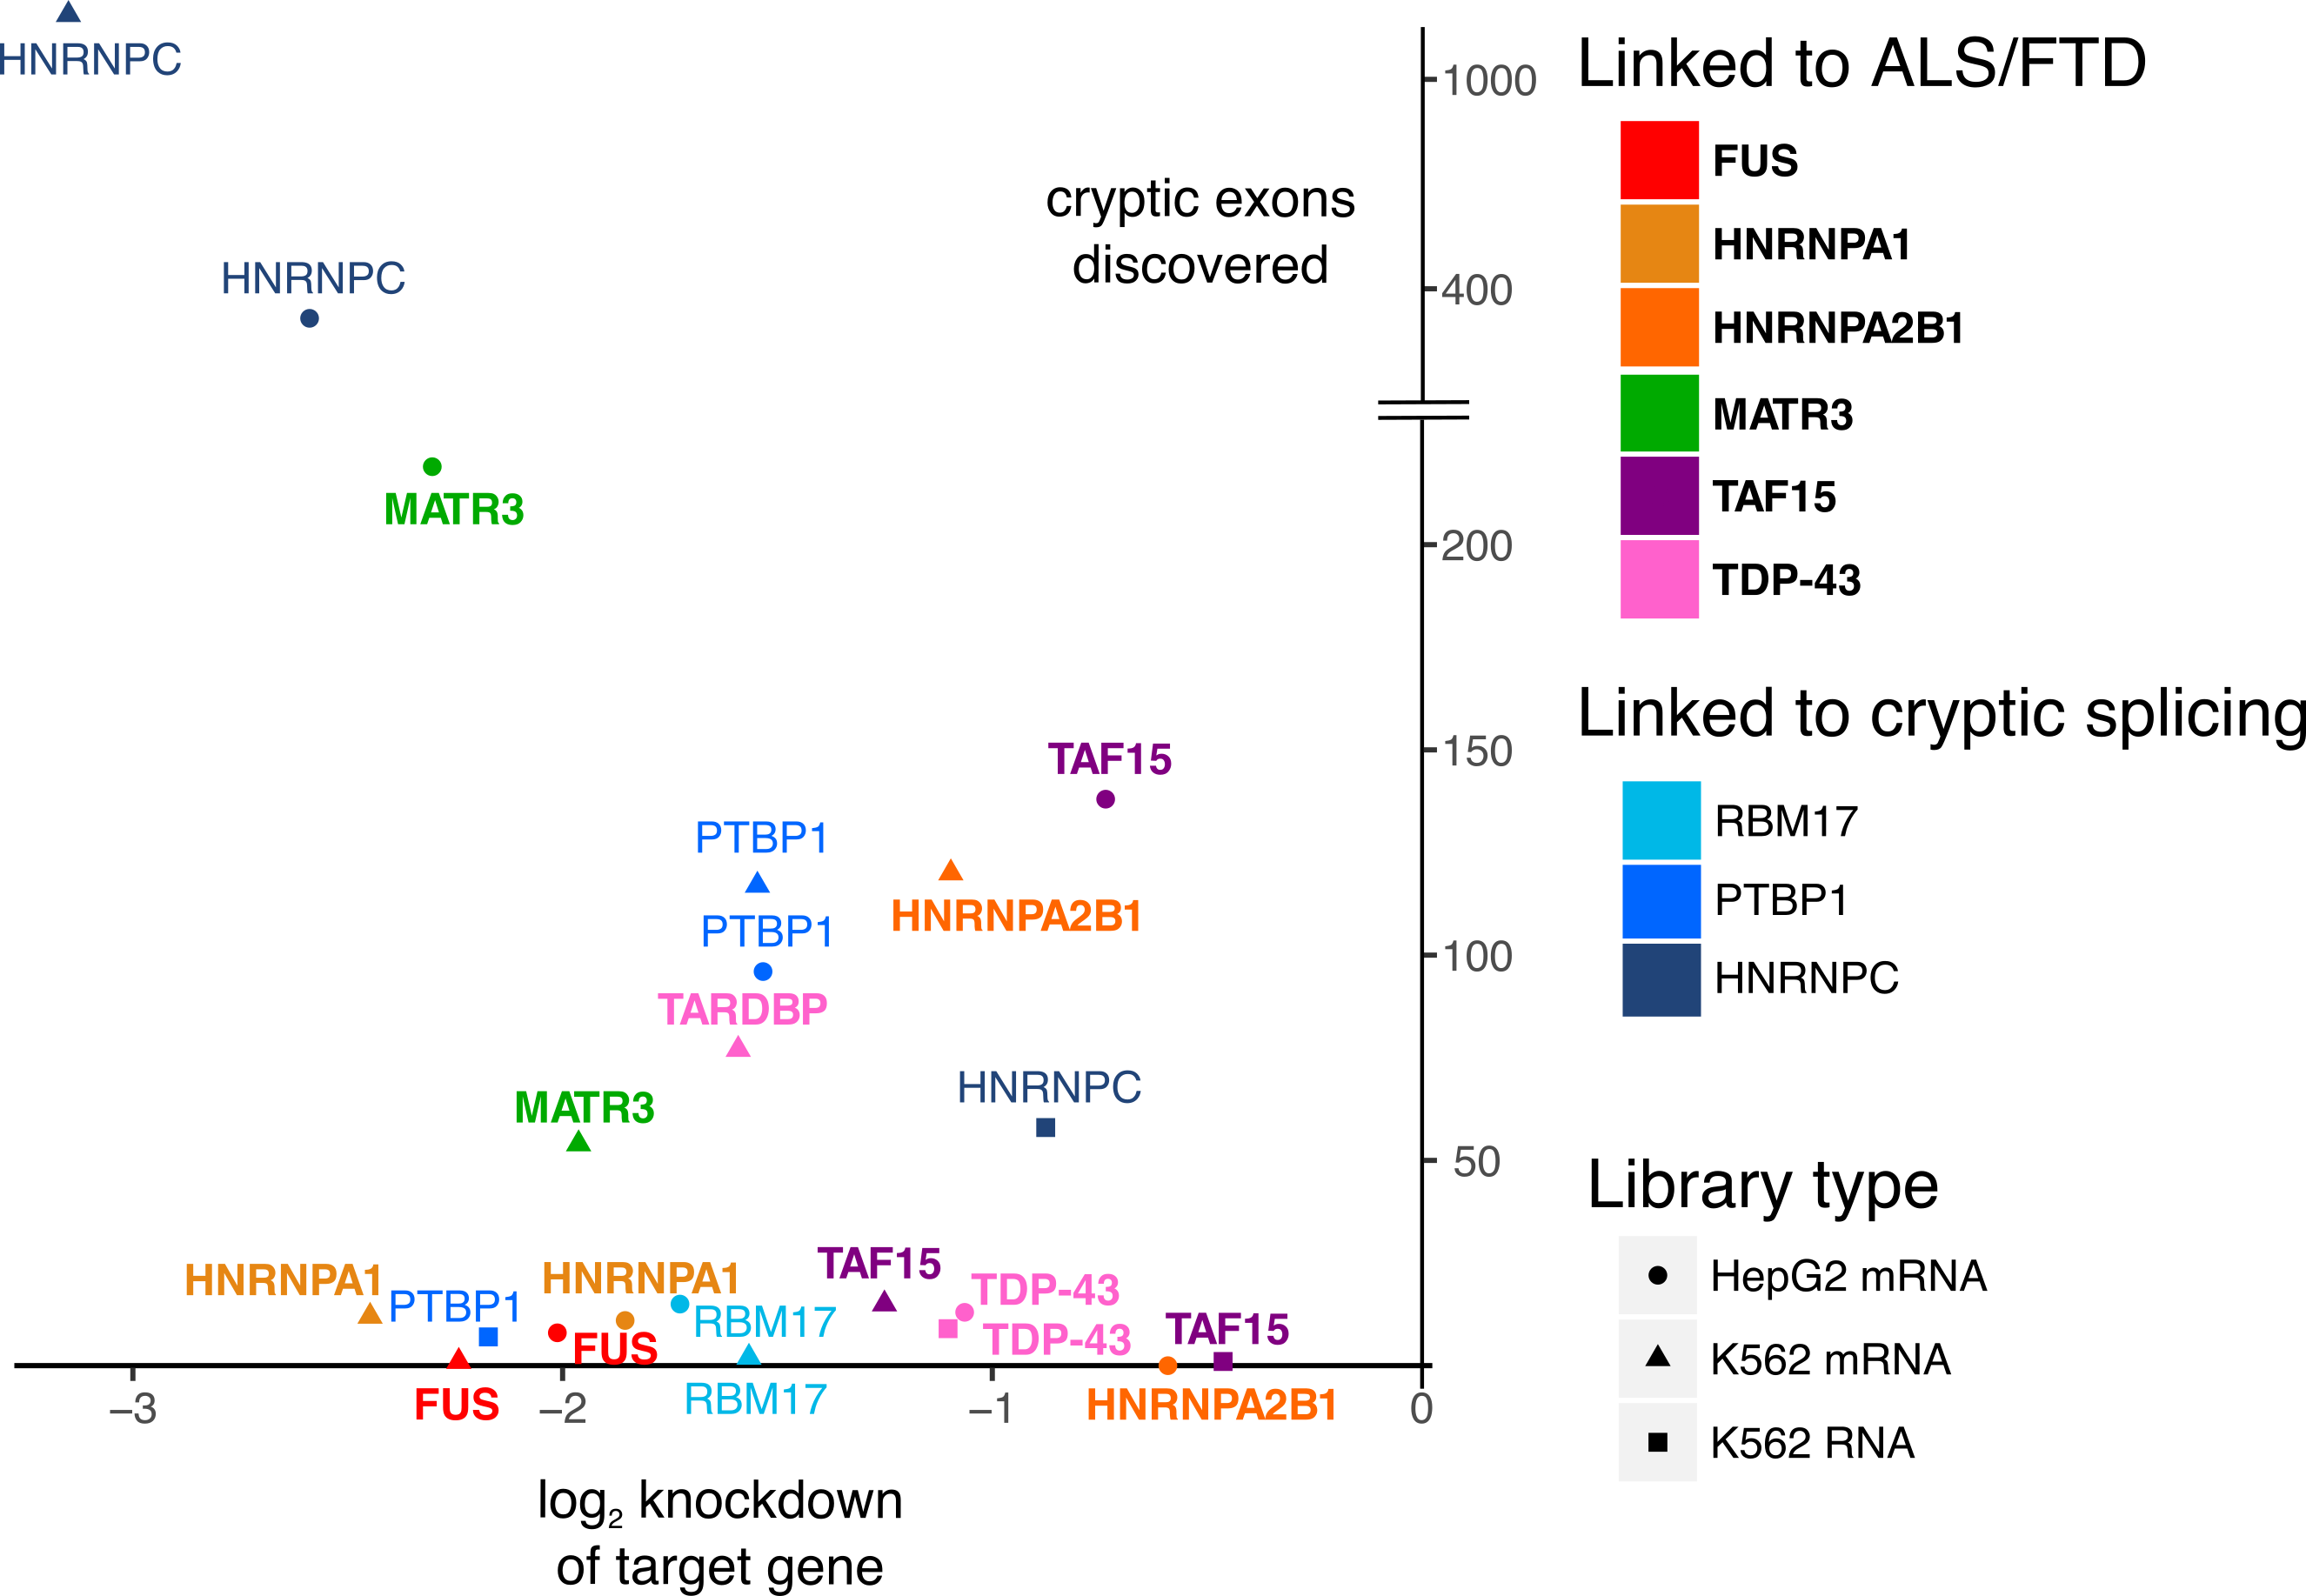
\includegraphics[width=12cm]{Figures/ENCODE_summary.png}
	\end{center}
	\caption{ALS and cryptic splicing linked protein knockdowns from the ENCODE consortium  }
\end{figure} 

\section{Cryptic splicing in ALS and FTD patient brain}
The initial paper on TDP-43 and cryptic splicing observed that two cryptic exons out of the 50 observed in HeLa cells could also be observed in the brains of ALS patients but not in non-neurological disease controls \citep{Ling2015}. Since then no further work has studied cryptic splicing in ALS or FTD brains. There are multiple lines of evidence that suggest that a number of RNA-binding proteins are perturbed in ALS/FTD as well as TDP-43 and FUS. Therefore if all the potential cryptic targets were known for a host of RNA binding proteins, the inclusion of these cryptic exons in diseased brain would suggest a perturbation in expression of that protein. 
Building on the results of the TDP-43 cryptic splicing project and the results of the ENCODE screen, I want to thoroughly search for evidence of cryptic splicing in a set of control and disease brains. One such set of sporadic and familial ALS brain RNA-seq data has been previously published \citep{Prudencio2015}. We also have an in-house set of FTD and control brain RNA-seq (unpublished). The data will need to be very carefully prepared. I will attempt to deconvolute gene expression by cell type to compare the levels of neurons and glial cells in the control and diseased brains, to better understand differences in splicing changes between disease samples. RNA-seq of purified cells is available in mouse \citep{Newman2016} and algorithms for this specific task have been developed \citep{Zhang2014}. This approach has successfully applied to human brains to investigate cell type changes in aging \citep{Soreq2017}. There is also scope to look in patient blood and cerebrospinal fluid for potential RNA biomarkers to track disease course. 

\section{Conclusions}
My work so far has investigated RNA regulation in models of both sporadic and genetic ALS/FTD. Completion of my PhD should result in a fuller picture of cryptic splicing as a general mechanism of disease, complemented by a fine-grained analysis of specific mutations in \textit{TARDBP} and \textit{FUS}. Taking these insights into human patient tissue will be challenging but may lead to advances in understanding both ALS and FTD. 

